% Unofficial UofT Poster template.
% A fork of the UMich template https://www.overleaf.com/latex/templates/university-of-michigan-umich-poster-template/xpnqzzxwbjzc
% which is fork of the MSU template https://www.overleaf.com/latex/templates/an-unofficial-poster-template-for-michigan-state-university/wnymbgpxnnwd
% which is a fork of https://www.overleaf.com/latex/templates/an-unofficial-poster-template-for-new-york-university/krgqtqmzdqhg
% which is a fork of https://github.com/anishathalye/gemini
% also refer to https://github.com/k4rtik/uchicago-poster

\documentclass[final]{beamer}

% ====================
% Packages
% ====================

\usepackage[T1]{fontenc}
 \usepackage[utf8]{luainputenc}
\usepackage{lmodern}
\usepackage[size=custom, width=122,height=91, scale=1.2]{beamerposter}
\usetheme{gemini}
\usecolortheme{uoft}
\usepackage{graphicx}
\usepackage{booktabs}
\usepackage{tikz}
\usepackage{pgfplots}
\pgfplotsset{compat=1.14}
\usepackage{anyfontsize}

\usepackage{tikz}
\usetikzlibrary{decorations.pathreplacing}

% ====================
% Lengths
% ====================

% If you have N columns, choose \sepwidth and \colwidth such that
% (N+1)*\sepwidth + N*\colwidth = \paperwidth
\newlength{\sepwidth}
\newlength{\colwidth}
\setlength{\sepwidth}{0.025\paperwidth}
\setlength{\colwidth}{0.3\paperwidth}

\newcommand{\separatorcolumn}{\begin{column}{\sepwidth}\end{column}}

% ====================
% Title
% ====================

\title{Neural Style Transfer: Fundamental Theory and Architecture}

\author{Jingwen (Steven) Shi}

\institute[shortinst]{University of Toronto}

% ====================
% Footer (optional)
% ====================

\footercontent{
  \href{https://github.com/jingwenshi-dev/NST-Poster}{Github: https://github.com/jingwenshi-dev/NST-Poster} \hfill
CSC490 2023 Fall \hfill
  \href{mailto:jingwensteven.shi@mail.utoronto.ca}{jingwensteven.shi@mail.utoronto.ca}}
% (can be left out to remove footer)

% ====================
% Logo (optional)
% ====================

% use this to include logos on the left and/or right side of the header:
% Left: institution
 \logoright{
\includegraphics[height=8cm]{logos/logo.png}}
% Right: funding agencies and other affilations 
%\logoright{\includegraphics[height=7cm]{logos/NSF.eps}}
% ====================
% Body
% ====================

\begin{document}
\begin{frame}[t]
\begin{columns}[t]
\separatorcolumn

\begin{column}{\colwidth}

    \begin{block}{Abstract}
    
        This poster aims to provide a comprehensive overview of key concepts in neural style transfer including architecture, loss functions, transfer learning, target detaching, and layer choices.
    
    \end{block}

    \begin{block}{Architecture}
    
        Based on the VGG-19 pre-trained model with style loss and content loss layers inserted:
        
        \begin{itemize}
            \item Normalization
            \item Convolution
                \tikz[remember picture] \node[coordinate,xshift=1em,yshift=1em] (n1) {}; 
            \item ReLU
                \tikz[remember picture] \node[coordinate] (n2) {};
            \item \textbf{\textcolor{red} {Style Loss}}
                \tikz[remember picture] \node[coordinate] (n3) {};
            %%% Rander bracket for the set of items n1-n3 above %%%
            \begin{tikzpicture}[overlay,remember picture]
              \path (n3) -| node[coordinate] (n4) {} (n1);
              \draw[thick,decorate,decoration={brace,amplitude=10pt,aspect=0.5}]
                    (n1) -- (n4) node[midway, right=0.5em] {x2};
            \end{tikzpicture}
            %======================================================
            \item Max Pooling
            \item Convolution
                \tikz[remember picture] \node[coordinate,xshift=1em,yshift=1em] (n4) {}; 
            \item ReLU
                \tikz[remember picture] \node[coordinate] (n5) {};
            \item \textbf{\textcolor{red} {Style Loss}}
                \tikz[remember picture] \node[coordinate] (n6) {};
            %%% Rander bracket for the set of items n4-n7 above %%%
            \begin{tikzpicture}[overlay,remember picture]
              \path (n6) -| node[coordinate] (n7) {} (n4);
              \draw[thick,decorate,decoration={brace,amplitude=10pt,aspect=0.5}]
                    (n4) -- (n7) node[midway, right=0.5em] {x2};
            \end{tikzpicture}
            %======================================================
            \item \textbf{\textcolor{blue} {Content Loss}}
            \item Max Pooling
            \item Convolution
            \item ReLU
            \item \textbf{\textcolor{red} {Style Loss}}
        \end{itemize}
        
        The model does not include all the layers of VGG-19. In fact, the model got cut off and abandoned all the layers after the last loss layer was inserted for several reasons:
        \begin{itemize}
            \item \textbf{Focus on Style Features:\\}
            Neural style transfer aims to merge the content of an image with the style of another. By cutting off the model after the last loss layer, the model can focus on the style feature better and the rest of the VGG-19 layers are simply not helpful.
            \item \textbf{Computation Efficiency:\\}
            VGG-19 is a type of CNN model, the more layers a model has, the more computing-intensive it is. By cutting off the model, the layers are not necessarily for capturing content and style will not be computed.
        \end{itemize}
        
        \begin{figure}
          \centering
            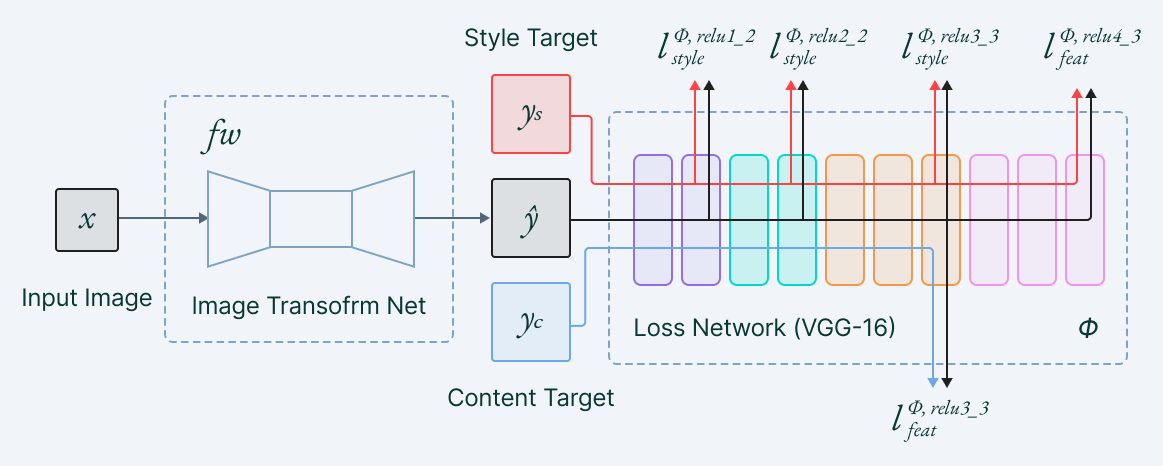
\includegraphics[width=0.75\textwidth]{figures/NST Architecture.png}
        
            \caption{Neural Style Transfer Architecture (source: V7 Labs)}
        \end{figure}
    
    \end{block}

\end{column}

\separatorcolumn

\begin{column}{\colwidth}

  \begin{alertblock}{Losses}

    The complete loss is the sum of the content and style loss since the goal is to minimize the joint losses on the generated image.

    $$
    \mathcal{L}_{total}(p, a, x) = \alpha\mathcal{L}_{content}(p, x) + \beta\mathcal{L}_{style}(a, x)
    $$
    where:
    \begin{itemize}
        \item $\alpha$ and $\beta$ are weighting factors that determine the relative importance of the content and style.
        \item p, a, x are the content, style, and input images.
    \end{itemize}

  \end{alertblock}

  \begin{block}{Content Loss}

    Each content loss is the mean square error (MSE) between the feature representation of content and the input image. It measures the difference between the generated image and the content image.

    $$\mathcal{L}_{content}(p, x, l) = \frac{1}{n} \sum_{i, j}(F^l_{i, j}(x) - F^l_{i, j}(p))^2$$
    where:
    \begin{itemize}
        \item $F^l_{i, j}$ is the feature map at layer l.
    \end{itemize}

  \end{block}

  \begin{block}{Style Loss}

    Style loss uses the same methodology as the content loss for calculation except now it has an additional step of calculation Gram matrix before before input to the MSE.
    
    $$\mathcal{L}_{content}(a, x, l) = \frac{1}{4 N^2_l M^2_l} \sum (G^l(x) - G^l(a))^2 $$
    where:
    \begin{itemize}
        \item $G^l$ is the Gram matrix of the feature map at layer $l$.
        \item $N_l$ is the number of feature maps at layer $l$.
        \item $M_l$ is the size of each feature map at layer $l$.
    \end{itemize}

  \end{block}


  \begin{block}{Why not Covariance Matrix?}

    Etiam sit amet tempus lorem, aliquet condimentum velit. Donec et nibh
    consequat, sagittis ex eget, dictum orci. Etiam quis semper ante. Ut eu
    mauris purus. Proin nec consectetur ligula. Mauris pretium molestie
    ullamcorper. Integer nisi neque, aliquet et odio non, sagittis porta justo.

    \begin{itemize}
      \item \textbf{Sed consequat} id ante vel efficitur. Praesent congue massa
        sed est scelerisque, elementum mollis augue iaculis.
        \begin{itemize}
          \item In sed est finibus, vulputate
            nunc gravida, pulvinar lorem. In maximus nunc dolor, sed auctor eros
            porttitor quis.
          \item Fusce ornare dignissim nisi. Nam sit amet risus vel lacus
            tempor tincidunt eu a arcu.
          \item Donec rhoncus vestibulum erat, quis aliquam leo
            gravida egestas.
        \end{itemize}
      \item \textbf{Sed luctus, elit sit amet} dictum maximus, diam dolor
        faucibus purus, sed lobortis justo erat id turpis.
      \item \textbf{Pellentesque facilisis dolor in leo} bibendum congue.
        Maecenas congue finibus justo, vitae eleifend urna facilisis at.
    \end{itemize}

  \end{block}

\end{column}

\separatorcolumn

\begin{column}{\colwidth}

  \begin{exampleblock}{A highlighted block containing some math}

    A different kind of highlighted block.

    $$
    \int_{-\infty}^{\infty} e^{-x^2}\,dx = \sqrt{\pi}
    $$

    Interdum et malesuada fames $\{1, 4, 9, \ldots\}$ ac ante ipsum primis in
    faucibus. Cras eleifend dolor eu nulla suscipit suscipit. Sed lobortis non
    felis id vulputate.

    \heading{A heading inside a block}

    Praesent consectetur mi $x^2 + y^2$ metus, nec vestibulum justo viverra
    nec. Proin eget nulla pretium, egestas magna aliquam, mollis neque. Vivamus
    dictum $\mathbf{u}^\intercal\mathbf{v}$ sagittis odio, vel porta erat
    congue sed. Maecenas ut dolor quis arcu auctor porttitor.

    \heading{Another heading inside a block}

    Sed augue erat, scelerisque a purus ultricies, placerat porttitor neque.
    Donec $P(y \mid x)$ fermentum consectetur $\nabla_x P(y \mid x)$ sapien
    sagittis egestas. Duis eget leo euismod nunc viverra imperdiet nec id
    justo.

  \end{exampleblock}

  \begin{block}{Nullam vel erat at velit convallis laoreet}

    Class aptent taciti sociosqu ad litora torquent per conubia nostra, per
    inceptos himenaeos. Phasellus libero enim, gravida sed erat sit amet,
    scelerisque congue diam. Fusce dapibus dui ut augue pulvinar iaculis.

    \begin{table}
      \centering
      \begin{tabular}{l r r c}
        \toprule
        \textbf{First column} & \textbf{Second column} & \textbf{Third column} & \textbf{Fourth} \\
        \midrule
        Foo & 13.37 & 384,394 & $\alpha$ \\
        Bar & 2.17 & 1,392 & $\beta$ \\
        Baz & 3.14 & 83,742 & $\delta$ \\
        Qux & 7.59 & 974 & $\gamma$ \\
        \bottomrule
      \end{tabular}
      \caption{A table caption.}
    \end{table}

    Donec quis posuere ligula. Nunc feugiat elit a mi malesuada consequat. Sed
    imperdiet augue ac nibh aliquet tristique. Aenean eu tortor vulputate,
    eleifend lorem in, dictum urna. Proin auctor ante in augue tincidunt
    tempor. Proin pellentesque vulputate odio, ac gravida nulla posuere
    efficitur. Aenean at velit vel dolor blandit molestie. Mauris laoreet
    commodo quam, non luctus nibh ullamcorper in. Class aptent taciti sociosqu
    ad litora torquent per conubia nostra, per inceptos himenaeos.



  \end{block}

  \begin{block}{References}

    \nocite{*}
    \footnotesize{\bibliographystyle{plain}\bibliography{poster}}

  \end{block}

\end{column}

\separatorcolumn
\end{columns}
\end{frame}

\end{document}
